\documentclass[conference,compsoc]{IEEEtran}
 
\usepackage{hyperref}
\usepackage{datetime}
\usepackage[table]{xcolor}
\usepackage{dsfont}
\usepackage{float}
\restylefloat{table}
\usepackage{pgfplots}
\pgfplotsset{width=8cm,compat=1.9}
\usepackage{graphicx}
\graphicspath{{./figures/}}
\usepackage{multirow}
\usepackage{enumitem}
\usepackage{bm}
\usepackage{amsmath}
\usepackage{tikz}
\usepackage{subfig}
\usetikzlibrary{positioning, fit, arrows.meta, shapes, arrows}
\newcommand{\empt}[2]{$#1^{\langle #2 \rangle}$}

\newenvironment{normalize}{\leftskip-\leftmargin}{\par}
\usepackage{listings}
\usepackage{xcolor}

\definecolor{codegreen}{rgb}{0,0.6,0}
\definecolor{codegray}{rgb}{0.5,0.5,0.5}
\definecolor{codepurple}{rgb}{0.58,0,0.82}
\definecolor{backcolour}{rgb}{0.95,0.95,0.92}

\lstdefinestyle{mystyle}{
    language=python,
    backgroundcolor=\color{backcolour},   
    commentstyle=\color{codegreen},
    keywordstyle=\color{magenta},
    numberstyle=\tiny\color{codegray},
    stringstyle=\color{codepurple},
    basicstyle=\ttfamily\footnotesize,
    breakatwhitespace=false,         
    breaklines=true,                 
    captionpos=b,                    
    keepspaces=true,                 
    numbers=left,                    
    numbersep=5pt,                  
    showspaces=false,                
    showstringspaces=false,
    showtabs=false,                  
    tabsize=2
}
\lstset{style=mystyle}

\usetikzlibrary{positioning}
\tikzstyle{inputNode}=[draw,circle,minimum size=10pt,inner sep=0pt]
\tikzstyle{stateTransition}=[-stealth, thick]

% *** CITATION PACKAGES ***
\ifCLASSOPTIONcompsoc
  \usepackage[nocompress]{cite}
\else
  \usepackage{cite}
\fi

% correct bad hyphenation
\hyphenation{op-tical net-works semi-conduc-tor}

\pagestyle{plain} % show number of pages

\setcounter{secnumdepth}{4}


\begin{document}

\title{BSP S3 - Speech Recognition for Luxembourgish by a Recurrent Neural
Network\\
{\small \today~-~\currenttime}}

\author{\IEEEauthorblockN{Le Minh Nguyen}
        \IEEEauthorblockA{University of Luxembourg\\
                Email: le.nguyen.001@student.uni.lu}
        \and
        \IEEEauthorblockN{Vladimir Despotovic}
        \IEEEauthorblockA{University of Luxembourg\\
                Email: vladimir.despotovic@uni.lu}
}

\maketitle


\textcolor{gray}{The length of the report should be from 6000 to 8000 words
  excluding images and annexes. The sections presenting the technical and
  scientific deliverables represent $\pm$ 80\% of total words of the report.}\\

\begin{abstract}

Recurrent neural networks (RNN) in comparison with conventional feedforward
neural networks, use their internal state to operate on data series. One of the
domains in which RNNs are applied is speech recognition. In this paper, the
focus will be on the classification of spoken words to their according labels.
We apply RNN, Long short-term memory (LSTM) and feedforward neural networks for
the classification and compare their accuracies.

\end{abstract}


\IEEEpeerreviewmaketitle

\section{Introduction ($\pm$ 5\% of total words)}

This paper presents the Bachelor Semester Project (BSP) made by Le Minh Nguyen
together with Vladimir Despotovic as his motivated tutor. The project is divided
into two periods. In the first period, we implement our classification model to
recognize spoken words. The first period contains the following concepts:\\

\begin{itemize}
\item Data preprocessing.
\item Training set and testing set.
\item Deep Neural Networks architecture: Deep Feedforward Neural Networks and
  Recurrent Neural Networks, which are presented in the popular Deep Learning textbook
  \cite{Goodfellow-et-al-2016}.
\end{itemize}

In the second period, we explain the deep Neural Networks architecture and compare their
accuracies obtained during our classification experiment.\\

\textcolor{gray}{The length of the report should be from 6000 to 8000 words
  excluding images and annexes. The sections presenting the technical and
  scientific deliverables represent $\pm$ 80\% of total words of the report.}

% correcte VD

\section{Project description}
\subsection{Domains}

\begin{itemize}
        \item Speech Recognition
        \item Artificial Neural Networks
        \item Deep Learning 
        \item Data preprocessing
        \item Training set and testing set
        \item Python
        \item Keras
\end{itemize}

\subsubsection{Scientific}

The scientific aspects covered by this Bachelor Semester Project are the
concepts of speech recognition and Deep Learning. Different Artificial Neural
Networks (ANN) architectures are investigated for the end-to-end isolated word
recognition task.\\

\textbf{Speech Recognition.} The objective of speech recognition is to map an
audio signal which contains a set of spoken natural language expressions to the
matching sequence of words produced by the speaker. In the past, Automatic
Speech Recognition (ASR) was made up of different modules such as complex
feature extraction, acoustic models, language and pronunciation
models.~\cite{DBLP:journals/corr/AmodeiABCCCCCCD15} Sequential models, such as
Hidden Markov Models (HMM), in combination with a pre-trained language model,
were used to map sequences of phones to output words.~\cite{Williamsong} A
different approach is to build ASR models end-to-end. With deep learning, it
replaces most of the modules with a single module. This alternative method is
the main task of this report.\\

\textbf{Artificial Neural Networks (ANN).} ANNs are computing systems inspired
by the biological brain. These systems are based on a set of connected units
called artificial neurons. Each connection can transmit \textit{signals} between
units. A unit can process the signal and transmit it to another unit.\\

\textbf{Deep Learning.} This field deals with learning by decomposing a task's
input into smaller and simpler compositions. With Deep Learning, computing
systems can build complex concepts from a composition of simpler concepts.

\subsubsection{Technical} The technological aspect which is covered in this
project is the data collection, feature extraction and implementation of the
end-to-end spoken word recognition model. \\

\textbf{Data preprocessing.} Data preprocessing is an important phase in machine
learning. It ensures the quality of the gathered data by eliminating irrelevant
and redundant information. Data preprocessing contains tasks such as cleaning,
instance selection, normalization, feature extraction and feature selection. We
will focus on feature extraction in this paper with the presentation of
Mel-frequency cepstral coefficients (MFCCs) in Section~\ref{mfccs} which are
used as features extracted from the speech signal.\\

%add section

\textbf{Training set and testing set.} For a computing system to learn from and
make predictions on data, a mathematical model is built from input data. This
input data used to create the model consists of two datasets: The training and
testing set. The training set contains pairs of an input vector, which represent
features and an output vector often called the labels. With the training set,
the model learns to map the input vector to the labels. On the other hand, the
testing set evaluates how well the model generalizes the prediction over the
dataset previously not seen by the model.\\

\textbf{Python.} This is a programming language which is interpreted, high-level
and general-purpose.~\cite{Python}\\

\textbf{Keras Library.} \textit{Keras} is a high-level Neural Networks API
written in Python. It is designed for easy-to-use and efficient experimentation
with Deep Learning.~\cite{chollet2015keras}

\subsection{Targeted Deliverables}

\subsubsection{Scientific deliverables}

% Scientific
% -fnn
% -rnn
% -lstm
% -data preprocessing with mfcc
% -accuracy comparison

% Technical
% -model implementation
% -luxembourgish data collection

One of the main deliverables is to present the notions of deep learning. This
paper should give a small introduction to Neural networks and their application
for classification. Further, we extend this scientifical presentation by diving
deeper into three different Neural Networks; Feedforward Neural Networks,
Recurrent Neural Networks (RNN) and Long short-term memory (LSTM). Additionally,
we explain how we extract the features from the dataset. Finally, we compare
their accuracies obtained after being trained on the given audio dataset.\\

\textcolor{gray}{Provide a synthetic and abstract description of the scientific
deliverables that were targeted to be produced.}

\subsubsection{Technical deliverables} 

The other main deliverable for this paper is to implement our classification
model based on the three Neural Networks mentioned in the section above.
Additionally, we collect a small dataset of Luxembourgish spoken words $w \in
\{'0',...,'9','moien'\}$ to train our model to classify these words.\\ 

\textcolor{gray}{Provide a synthetic and abstract description of the technical
deliverables that were targeted to be produced.}

%corrected

\subsection{Constraints}

For this BSP, we set the different constraints for the ANNs, for the speech
recognition, for the Luxembourgish vocal dataset and the classification model's
implementation.\\

\textbf{Data set.} First, we focus on training our model on a dataset
containing English spoken numbers.~\cite{DBLP:journals/corr/abs-1804-03209}
After having trained the model successfully on this dataset, we train it on the
smaller Luxembourgish dataset and analyse its prediction accuracy. Since we
aren't able to collect as much voice recordings as the English data set, we
should not expect high accuracy.\\

%reference paper

\textbf{Speech recognition.} Since no datasets with continuous sentences of the
Luxembourgish Language exists, we choose to work with isolated word recognition
instead of continuous speech recognition. In isolated word recognition, words are
separated by pauses.\\

\textbf{Speaker dependency.} To simplify the collection of the Luxembourgish
dataset, we collect the audio recordings from one person which makes the
isolated word recognition speaker-dependent.\\

\textbf{ANNs implementation.} We do not implement the Artificial Neural Networks
architecture since existing deep learning libraries such as Keras are already
matured. Thereby, we focus on explaining how the APIs work and how to use them
efficiently in our model.

% corrected VD

\section{Pre-requisites} 

To start on the project, certain skills in programming and mathematics are
required. In particular, the preliminary requirement of the project is as
follows:~\\
\begin{itemize}
        \item Understanding of vector and matrix algebra.
        \item Introductory course in Python.
        \item Software development.
        \item Knowledge of probability and statistics is desirable although not
          mandatory.
\end{itemize}

\subsection{Scientific pre-requisites}

\textbf{Linear Algebra.} is a sub-field of mathematics, which works with vectors
and matrices. Since the input of deep learning is data that are transformed into
structures of rows and columns, linear algebra is one of the key foundations of
deep learning. It is used to describe the operations of the deep learning
algorithms, and implement the algorithms in code. All tasks in deep learning
relate to linear algebra, from data preprocessing to the deep learning
algorithms.~\cite{Goodfellow-et-al-2016}

\subsection{Technical pre-requisites}

\textbf{Python.} Python is an interpreted, high-level and general-purpose
programming language, which is conceived in the late 1980s and released in 1991
by Guido van Rossum.~\cite{PyRo} Its design philosophy accentuates readability
of the code.  As many high-level programming languages, Python is dynamically
typed. Further, it supports multiple programming paradigms such as procedural,
object-oriented and functional programming. With a proficient background in
programming in Python gained during my high school and university education, I
am prepared to work on this project.\\

\textbf{Software development.} Software development is the process of designing
and implementation of applications and frameworks. In general, the process of
software development includes writing and maintaining the source code which is
often a planned and structured process. The software development contains mostly
research, prototyping, modification and reuse of existing software. During the
technical deliverable section, we use this structured process to design and
implement our ANNs. 

% corrected LN 84

\section{Scientific Deliverables}

The scientific deliverables are the following; the feature extraction with MFCCs
are presented, notions of deep learning and Artificial Neural Networks (ANNs)
will be investigated. This section will wrap up by a performance evaluation of
four different ANNs models.

% corrected VD 97

\subsection{Requirements}
% Describe here all the properties that characterize the deliverables you
% produced. It should describe, for each main deliverable, what are the expected
% functional and non functional properties of the deliverables, who are the actors
% exploiting the deliverables. It is expected that you have at least one
% scientific deliverable (e.g. ``Scientific presentation of the Python programming
% language'', ``State of the art on quality models for human computer
% interaction'', \ldots.) and one technical deliverable (e.g. ``BSProSoft - A
% python/django web-site for IT job offers retrieval and analysis'', \ldots). \\

\begin{itemize} 
  \item \textbf{FR01} Present the feature extraction with MFCCs \\
  \item \textbf{FR02} Investigate the notions of deep learning and Artificial
    Neural Networks (ANNs)\\
    This should give an introduction to the domain of deep learning. It presents
    an overview of 3 different ANNs architectures, namely every Neural Network
    presentation will cover a small introduction and theoretical aspect.\\
  \item \textbf{NFR01} Performance evaluation and comparison\\ 
    During this section, we present and discuss the results obtained using
    three Neural Network architectures.
\end{itemize}

% corrected

\subsection{Design}

% corrected VD 81

\subsubsection{FR01: Feature extraction with MFCCs}\label{mfccs}~\\

% introduction

Before training our end-to-end ASR model, audio data have to be preprocessed.
The first task is to extract features from the data which describes natural
language expressions and excludes background noises and emotions.\\

% def of MFCCs

Mel Frequency Cepstral Coefficients (MFCCs) are features widely used in ASR.
MFCCs were presented by Davis and Mermelstein in the 1980s.~\cite{mfcc}\\

To extract the MFCCS from the dataset, the following extraction steps have to be
executed on a speech signal sampled at $16kHz$:\\

\begin{enumerate}[label=\arabic*.]
  \item Frame the signal into $25ms$ frames. The frame length of a $16kHz$
    signal:
  \begin{equation} 
    0.025*16000 = 400 samples.
  \end{equation}
  With a frame step of $160\ samples$ or $10ms$, the frames overlap themselves,
  such that the first frame containing $400\ samples$ starts at sample 0 and the
  second frame starts at sample 160. This pattern repeats until the end of the
  speech signal. If the audio file is not divisible by an even number, it is
  padded by zeros.\\
  \item For each frame calculate the periodogram estimate of the power spectrum.
    To obtain the Discrete Fourier Transform (DFT) from the frame $i$, we
    perform:
    \begin{equation}
      S_{i}(k) = \sum_{N}^{n=1}s_i(n)h(n)e^{-j2\pi kn/N}
    \end{equation}
    For each speech frame $s_{i}(n)$, the periodogram-based power spectral
    estimate is calculated with:
    \begin{equation}
      P_{i}(k)=\frac{1}{N}{\mid{S_{i}(k)}\mid}^{2}
    \end{equation}
  This is called the Periodogram estimate of the power spectrum which identifies
  for every frame which frequencies are present.\\
  \item Apply the Mel filterbank to the power spectrum and sum the energy in
    each filter. The Mel filterbank is a set of 26 triangular filters. The
    filterbank energies are calculated by multiplying every filterbank with the
    power spectrum.\\
  \item Take the logarithm of the 26 filterbank energies.\\
  \item Take the Discrete Cosine Transform (DCT) of the 26 log filterbank
    energies resulting in 26 cepstral coefficients. We only used the lower 12-13
    of the 26 coefficients for ASR.\\
\end{enumerate}

In Section~\ref{librosa} we will use the Python library \textit{Librosa} to
extract the MFCCs features from the dataset.
 % corrected
% corrected LN 87

\subsubsection{FR02: Deep Learning and Artificial Neural Networks}~\\

The notions of Deep Learning and examples of ANNs presented in this section are
based on the textbook \textit{Deep Learning}\cite{Goodfellow-et-al-2016} written
by \textit{Ian Goodfellow, Yoshua Bengio and Aaron Courville}. These
presentations should only give a high-level introduction to these notions.

\subsubsection{Deep Learning}~\\

Artificial Intelligence (AI) is a field with many practical applications such as
understanding speech, etc. AI deals with challenging problems which are easy to
perform but hard to describe formally by humans. Deep Learning is a solution to
these intuitive problems. This approach to AI allows computer systems to study
from experience and understand the world through a hierarchal stack of concepts.
The computing system gathers knowledge from experience which eliminates the need
to describe formal rules. The computer understands complex concepts with this
stack of concepts by decomposing them with simpler ones. The representation of
this hierarchy of concepts shows a deep graph with many layers, hence the name
for Deep Learning.~\cite{Goodfellow-et-al-2016}
 % corrected
% corrected LN 94

\subsubsection{Feedforward Neural Network}~\\

Feedforward neural networks or multilayer perceptrons (MLPs) are very important
deep learning models. The objective of MLPs is to approximate a given function
$f^{*}$. A feedforward network defines a mapping $\bm{\hat{y}} = f(\bm{x};
\bm{\theta})$ and learns the values of the parameter $\bm{\theta}$ with a given
input vector $\bm{x}$ which yields the best approximation of $f^{*}$. This
function can be for example a classifier, $y = f^{*}(\bm{x})$ which maps an
input $\bm{x}$ to a class $y$.\\

These structures are called \textbf{feedforward} since there is a progress of
information. It is first evaluated as input $\bm{x}$ through the function
$\bm{f}$, then goes through the computations which define $\bm{f}$ and ends up
at the output $\bm{y}$.\\

MLPs are called \textbf{networks} because they are made up of composed
functions. Let $f_{1}$, $f_{2}$ and $f_{3}$ be three function forming a chain
$f(\bm{x}) = f_{3}(f_{2}(f_{1}(\bm{x})))$. The chain structures are commonly
used in ANNs. In the example, $f_{1}$ is called the first layer of the network,
$f_{2}$ is called the second layer, etc. The lenght of the chain represents the
depth of the network. The final layer is also called the output layer.\\

During the training of the neural network, we try to find $f(\bm{x})$ to
approximate $f^{*}(\bm{x})$. The training data contains examples of
$f^{*}(\bm{x})$ obtained with different training points where every example
$\bm{x}$ is referring to a label $y \approx f^{*}(\bm{x})$. These examples
determine how the output layer should approximate a value close to $y$ with each
example $\bm{x}$. The other layers are called the \textbf{hidden layers} because
the training examples are not determining their behaviour and it doesn't contain
the desired output of each layer. Therefore, a learning algorithm has to
determine how to utilize the hidden layers to obtain a good approximation of
$f^{*}(\bm{x})$.\\

The \textbf{width} of the feedforward model is defined by the dimensionality of
each hidden layer which is usually a vector containing values. These vector
layers can be thought of containing many \textbf{units} which process in
parallel. Each unit refers to a vector-to-scalar function, by taking input from
other units and calculating its proper activation value.\\

We will present a simple MLPs with one hidden layer which contains hidden units.
The hidden layer represents a vector of hidden units $\bm{h}$ which are
calculated by a function $f_{1}(\bm{x;\theta})$. $\bm{\theta}$ consists of
$\bm{W}$ and $\bm{B}$ which are the $weights$ and $biases$ repectively such
that:

\begin{equation}
  \begin{split}
    h & = f_{1}(\bm{x;W,B}) \\
    \Leftrightarrow h & = \bm{W}^{T}\bm{x}+\bm{B}
  \end{split}
\end{equation}

$\bm{h}$ is then used as input for the second layer which is the output layer;
$f_{2}(\bm{h;w,b})$. 

\begin{equation}
  \begin{split}
    y & = f_{2}(\bm{h;w,b}) \\
    \Leftrightarrow y & = \bm{w}^{T}\bm{h}+\bm{b}
  \end{split}
\end{equation}

The network can be illustrated as a chain of two functions:

\begin{equation} 
  f(\bm{x;W,B,w,b}) = f_{2}(f_{1}(\bm{x}))
\end{equation}

After using an affine transformation, the hidden units are computed by a
nonlinear function called an activation function:

\begin{equation} 
  h = g(\bm{W}^{T}\bm{x+B})
\end{equation}

The default activation function is the \textbf{rectified linear unit} or ReLU
defined as:

\begin{equation} 
  g(z) = \max\{0,z\}
\end{equation}

\begin{figure}[h]
  \centering
  \begin{tikzpicture}
      \begin{axis}[
          domain=-5:5,
          ylabel={$g(z) = \max\{0,z\}$}
          ]
          \addplot+[mark=none,blue,domain=-5:0] {0};
          \addplot+[mark=none,blue,domain=0:5] {x};
      \end{axis}
  \end{tikzpicture}
  \caption{The rectified linear activation function.}
\end{figure}


The complete feedforward network looks as follow:
\begin{equation} 
  f(\bm{x;W,B,w,b}) = \bm{w}^{T}\max\{0,\bm{W}^{T}\bm{x+B}\}+\bm{b}
\end{equation}

A representation of a single perceptron and its position in an MLP is given in
figure~\ref{mlp}.\\

\begin{figure}[h]
  \centering
  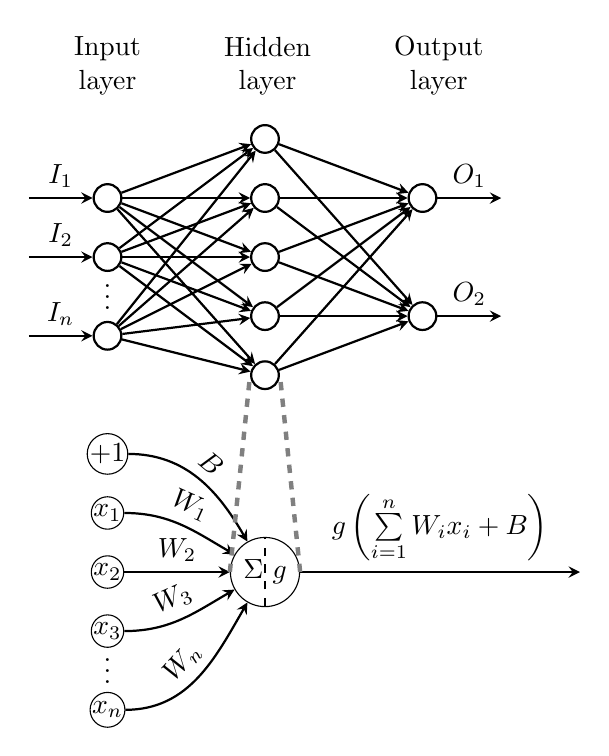
\begin{tikzpicture}
  % large MLP

  \node[inputNode, thick] (i1) at (-2, 0.75) {};
  \node[inputNode, thick] (i2) at (-2, 0) {};
  \node[inputNode, thick] (i3) at (-2, -1) {};
  \node (dots) at (-2, -0.4) {$\vdots$};

  \node[inputNode, thick] (h1) at (0, 1.5) {};
  \node[inputNode, thick] (h2) at (0, 0.75) {};
  \node[inputNode, thick] (h3) at (0, 0) {};
  \node[inputNode, thick] (h4) at (0, -0.75) {};
  \node[inputNode, thick] (h5) at (0, -1.5) {};

  \node[inputNode, thick] (o1) at (2, 0.75) {};
  \node[inputNode, thick] (o2) at (2, -0.75) {};

  \draw[stateTransition] (-3, 0.75) -- node[above] {$I_1$} (i1);
  \draw[stateTransition] (-3, 0) -- node[above] {$I_2$} (i2);
  \draw[stateTransition] (-3, -1) -- node[above] {$I_n$} (i3);

  \draw[stateTransition] (i1) -- (h1);
  \draw[stateTransition] (i1) -- (h2);
  \draw[stateTransition] (i1) -- (h3);
  \draw[stateTransition] (i1) -- (h4);
  \draw[stateTransition] (i1) -- (h5);
  \draw[stateTransition] (i2) -- (h1);
  \draw[stateTransition] (i2) -- (h2);
  \draw[stateTransition] (i2) -- (h3);
  \draw[stateTransition] (i2) -- (h4);
  \draw[stateTransition] (i2) -- (h5);
  \draw[stateTransition] (i3) -- (h1);
  \draw[stateTransition] (i3) -- (h2);
  \draw[stateTransition] (i3) -- (h3);
  \draw[stateTransition] (i3) -- (h4);
  \draw[stateTransition] (i3) -- (h5);

  \draw[stateTransition] (h1) -- (o1);
  \draw[stateTransition] (h1) -- (o2);
  \draw[stateTransition] (h2) -- (o1);
  \draw[stateTransition] (h2) -- (o2);
  \draw[stateTransition] (h3) -- (o1);
  \draw[stateTransition] (h3) -- (o2);
  \draw[stateTransition] (h4) -- (o1);
  \draw[stateTransition] (h4) -- (o2);
  \draw[stateTransition] (h5) -- (o1);
  \draw[stateTransition] (h5) -- (o2);

  \node[above=of i1, align=center] (l1) {Input \\ layer};
  \node[right=2.3em of l1, align=center] (l2) {Hidden \\ layer};
  \node[right=2.3em of l2, align=center] (l3) {Output \\ layer};

  \draw[stateTransition] (o1) -- node[above] {$O_1$} (3, 0.75);
  \draw[stateTransition] (o2) -- node[above] {$O_2$} (3, -0.75);

  %single perceptron

  \node[draw,circle,minimum size=25pt,inner sep=0pt] (x) at (0,0-4) {$\Sigma$ $g$};
  \node[inputNode] (x0) at (-2, 1.5-4) {$\tiny +1$};
  \node[inputNode] (x1) at (-2, 0.75-4) {$\tiny x_1$};
  \node[inputNode] (x2) at (-2, 0-4) {$\tiny x_2$};
  \node[inputNode] (x3) at (-2, -0.75-4) {$\tiny x_3$};
  \node[inputNode] (xn) at (-2, -1.75-4) {$\tiny x_n$};

  \draw[stateTransition] (x0) to[out=0,in=120] node [midway, sloped, above] {$B$} (x);
  \draw[stateTransition] (x1) to[out=0,in=150] node [midway, sloped, above] {$W_1$} (x);
  \draw[stateTransition] (x2) to[out=0,in=180] node [midway, sloped, above] {$W_2$} (x);
  \draw[stateTransition] (x3) to[out=0,in=210] node [midway, sloped, above] {$W_3$} (x);
  \draw[stateTransition] (xn) to[out=0,in=240] node [midway, sloped, above] {$W_n$} (x);
  \draw[stateTransition] (x) -- (4,0-4) node [midway,above]
    {$g\left(\sum\limits_{i=1}^{n}{W_ix_i} + B\right)$};
  \draw[dashed] (0,-0.43-4) -- (0,0.43-4);
  \node (dots) at (-2, -1.15-4) {$\vdots$};

  \path[dashed, double, ultra thick, gray] (x.west) edge[bend left=0] (h5.west);
  \path[dashed, double, ultra thick, gray] (x.east) edge[bend right=0] (h5.east);

  \end{tikzpicture}
  \label{mlp}
  \caption{A figure of a single perceptron with its position in a large-scale MLP.}
\end{figure}


\textbf{Gradient-Based Learning.} During the training of the model, deep
learning algorithms solve an optimization problem. The Problem is to minimize
some function $f(x)$ by changing its input $x$. This function is referred to as
the objective function also called the loss function. With the loss function the
deep learning model optimizes the approximation of $f^{*}$. An example of a loss
function for our MLP can be the mean squared error (MSE):

\begin{equation} 
  \frac{1}{n}\sum_{i=1}^n(f^*(\bm x_i)-f(\bm x_i;\bm{\theta}))^2
\end{equation}

ANNs usually used gradient-based optimizers to obtain a minimal loss function.\\

\textbf{Back-propagation.} We call forward propagation when an MLP takes
$\bm{x}$ as input and computes $\bm{\hat{y}}$ as output since the information
passes through the network. The back-propagation algorithm passes information
from the loss function backwards through the network. This algorithm computes
the gradient while passing back the network. With this gradient, another
algorithm called the \textit{stochastic gradient descent} performs the learning
of the $weight = \{W,w\}$ and the $biases = \{B,b\}$ and adjusts them to
minimize the lost function.
 % corrected
% corrected LN 93

\subsubsection{Recurrent Neural Network}~\\

%introduction
Recurrent Neural Networks (RNNs) are a particular architecture of ANNs which can
process sequential data $S = x^{(1)},\dots,x^{(\tau)}$. To explain how RNNs are
implemented, we have to introduce the notion of computational graphs.
A computational graph is a formal structure representing a set of computations.
We obtain a chain of events by unfolding a recurrent computation into a
computational graph with a repetitive structure. \\

Consider a recurrent system,
\begin{equation}
  s^{(t)} = f(s^{(t-1)};\theta)
\end{equation}
with $s$ being the state of the system. The graph can be unfolded considering
the time step $\tau = 3$, we have,
\begin{equation}
  \begin{split}
    s^{(3)} & = f(s^{(2)};\theta) \\
          & = f(f(s^{(1)};\theta);\theta)
  \end{split}
  \label{recurrentsystem}
\end{equation}
This expression can be illustrated by a directed acyclic computational graph.
See figure~\ref{dag}\\
\begin{figure}[h]
  \centering
  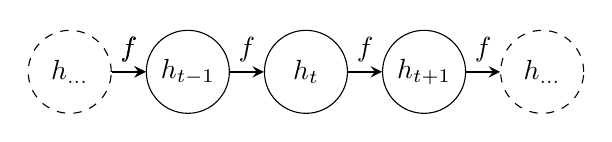
\begin{tikzpicture}
    \node[inputNode, dashed, minimum size=3em] (s0) at (-3,0) {$\tiny h_{\dots}$};
    \node[inputNode, minimum size=3em] (s1) at (-1.5,0) {$\tiny h_{t-1}$};
    \node[inputNode, minimum size=3em] (s2) at (0,0) {$\tiny h_{t}$};
    \node[inputNode, minimum size=3em] (s3) at (1.5,0) {$\tiny h_{t+1}$};
    \node[inputNode, dashed, minimum size=3em] (s4) at (3,0) {$\tiny h_{\dots}$};
    
    \draw[stateTransition] (s0) -- node[above] {$f$} (s1);
    \draw[stateTransition] (s0) -- node[above] {$f$} (s1);
    \draw[stateTransition] (s1) -- node[above] {$f$} (s2);
    \draw[stateTransition] (s2) -- node[above] {$f$} (s3);
    \draw[stateTransition] (s3) -- node[above] {$f$} (s4);

  \end{tikzpicture}
  \caption{The recurrent system described by equation \ref{recurrentsystem}, illustrated as an unfolded computational graph.}
  \label{dag}
\end{figure}


Now we consider recurrent system accepting an external signal $\bm{x}^{(t)}$,
\begin{equation}
  s^{(t)} = f(s^{(t-1)},\bm{x}^{(t)};\theta)
  \label{eqaccepting}
\end{equation}
where the state $s$ is containing information about the past sequence $S$. The
hidden units can be describe with equation~\ref{eqaccepting} using $\bm{h}$ to
denote the state,
\begin{equation}
  \bm{h}^{(t)} = f(\bm{h}^{(t-1)},\bm{x}^{(t)};\theta)
\end{equation}
represented in figure~\ref{unfoldrnnaccepting}.\\
\begin{figure}[h]
  \centering
  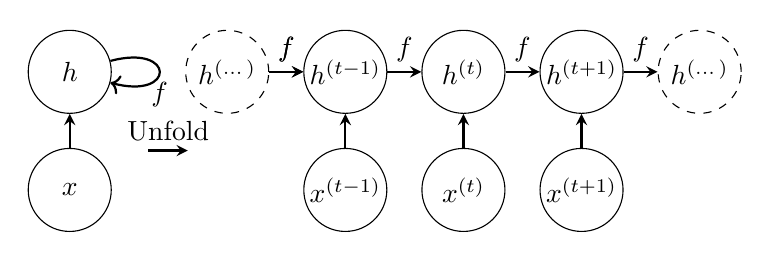
\begin{tikzpicture}

    \node[inputNode, minimum size=3em] (h) at (-5,0) {$\tiny h$};
    \node[inputNode, minimum size=3em] (x) at (-5,-1.5) {$\tiny x$};
    \node[inputNode, dashed, minimum size=3em] (s0) at (-3,0) {$\tiny h^{(\dots)}$};
    \node[inputNode, minimum size=3em] (s1) at (-1.5,0) {$\tiny h^{(t-1)}$};
    \node[inputNode, minimum size=3em] (s2) at (0,0) {$\tiny h^{(t)}$};
    \node[inputNode, minimum size=3em] (s3) at (1.5,0) {$\tiny h^{(t+1)}$};
    \node[inputNode, dashed, minimum size=3em] (s4) at (3,0) {$\tiny h^{(\dots)}$};
    \node[inputNode, minimum size=3em] (x1) at (-1.5,-1.5) {$\tiny x^{(t-1)}$};
    \node[inputNode, minimum size=3em] (x2) at (0,-1.5) {$\tiny x^{(t)}$};
    \node[inputNode, minimum size=3em] (x3) at (1.5,-1.5) {$\tiny x^{(t+1)}$};
    
    \draw[stateTransition] (x) -- (h);
    \draw[thick, ->, loop right] (h) to node[below] {$f$} (h);
    \draw[stateTransition] (-4,-1) -- node[above] {Unfold} (-3.5,-1);
    \draw[stateTransition] (s0) -- node[above] {$f$} (s1);
    \draw[stateTransition] (s0) -- node[above] {$f$} (s1);
    \draw[stateTransition] (s1) -- node[above] {$f$} (s2);
    \draw[stateTransition] (s2) -- node[above] {$f$} (s3);
    \draw[stateTransition] (s3) -- node[above] {$f$} (s4);
    \draw[stateTransition] (x1) -- (s1);
    \draw[stateTransition] (x2) -- (s2);
    \draw[stateTransition] (x3) -- (s3);

  \end{tikzpicture}
  \caption{This is an RNN with no outputs, it processes the input $x$ and passes
  it into the state $h$ which is then passed through time. On the right graph,
we have, the same network unfolded as a computational
graph.~\cite{Goodfellow-et-al-2016}}
  \label{unfoldrnnaccepting}
\end{figure}


%math

With graph unfolding, we can now present some common example of an RNNs. Here are
some important designs of RNNs:
\begin{itemize}
  \item RNNs which produce an output at every time step $\tau$ and are connected
    recurrently between hidden units.
  \item RNNs which produce an output at every time step $\tau$ and are connected
    recurrently only from the output from one time step between hidden units at
    another time step.
  \item RNNs which are connected recurrently between hidden units, read an
    entire data sequence $S$ and produce only one single output.
\end{itemize}

\begin{figure}[h]
  \centering
  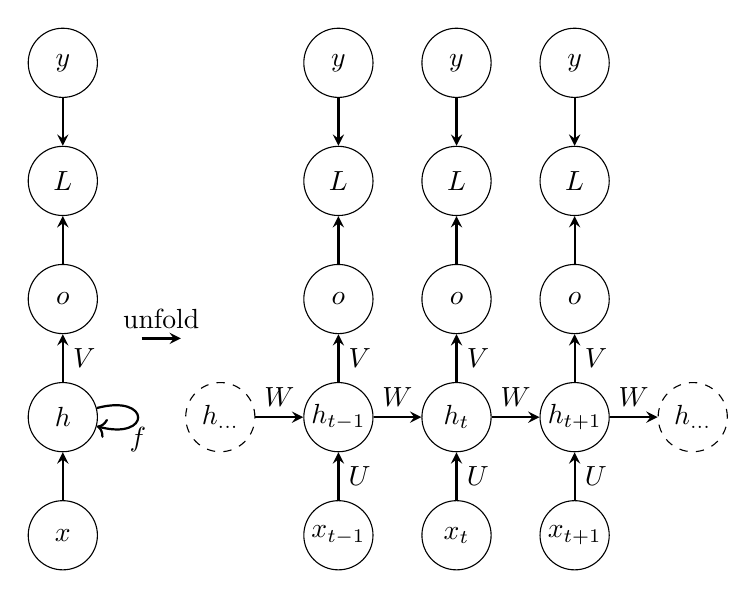
\begin{tikzpicture}

    % nodes

    \node[inputNode, minimum size=2.5em] (x0) at (-5,-1.5) {$\tiny x$};
    \node[inputNode, minimum size=2.5em] (h) at (-5,0) {$\tiny h$};
    \node[inputNode, minimum size=2.5em] (o0) at (-5,1.5) {$\tiny o$};
    \node[inputNode, minimum size=2.5em] (l0) at (-5,3) {$\tiny L$};
    \node[inputNode, minimum size=2.5em] (y0) at (-5,4.5) {$\tiny y$};



    \node[inputNode, dashed, minimum size=2.5em] (s0) at (-3,0) {$\tiny h_{\dots}$};

    \node[inputNode, minimum size=2.5em] (x1) at (-1.5,-1.5) {$\tiny x_{t-1}$};
    \node[inputNode, minimum size=2.5em] (s1) at (-1.5,0) {$\tiny h_{t-1}$};
    \node[inputNode, minimum size=2.5em] (o1) at (-1.5,1.5) {$\tiny o$};
    \node[inputNode, minimum size=2.5em] (l1) at (-1.5,3) {$\tiny L$};
    \node[inputNode, minimum size=2.5em] (y1) at (-1.5,4.5) {$\tiny y$};

    \node[inputNode, minimum size=2.5em] (x2) at (0,-1.5) {$\tiny x_{t}$};
    \node[inputNode, minimum size=2.5em] (s2) at (0,0) {$\tiny h_{t}$};
    \node[inputNode, minimum size=2.5em] (o2) at (0,1.5) {$\tiny o$};
    \node[inputNode, minimum size=2.5em] (l2) at (0,3) {$\tiny L$};
    \node[inputNode, minimum size=2.5em] (y2) at (0,4.5) {$\tiny y$};

    \node[inputNode, minimum size=2.5em] (x3) at (1.5,-1.5) {$\tiny x_{t+1}$};
    \node[inputNode, minimum size=2.5em] (s3) at (1.5,0) {$\tiny h_{t+1}$};
    \node[inputNode, minimum size=2.5em] (o3) at (1.5,1.5) {$\tiny o$};
    \node[inputNode, minimum size=2.5em] (l3) at (1.5,3) {$\tiny L$};
    \node[inputNode, minimum size=2.5em] (y3) at (1.5,4.5) {$\tiny y$};

    \node[inputNode, dashed, minimum size=2.5em] (s4) at (3,0) {$\tiny h_{\dots}$};

    
    % transition

    \draw[stateTransition] (x0) -- (h);
    \draw[thick, ->, loop right] (h) to node[below] {$f$} (h);

    \draw[stateTransition] (-4,1) -- node[above] {unfold} (-3.5,1);

    % \draw[stateTransition] (s0) -- node[above] {$f$} (s1);
    \draw[stateTransition] (s0) -- node[above] {$W$} (s1);
    \draw[stateTransition] (s1) -- node[above] {$W$} (s2);
    \draw[stateTransition] (s2) -- node[above] {$W$} (s3);
    \draw[stateTransition] (s3) -- node[above] {$W$} (s4);
    \draw[stateTransition] (o0) -- (l0);
    \draw[stateTransition] (y0) -- (l0);
    \draw[stateTransition] (o1) -- (l1);
    \draw[stateTransition] (y1) -- (l1);
    \draw[stateTransition] (o2) -- (l2);
    \draw[stateTransition] (y2) -- (l2);
    \draw[stateTransition] (o3) -- (l3);
    \draw[stateTransition] (y3) -- (l3);
    \draw[stateTransition] (x1) -- node[right] {$U$} (s1);
    \draw[stateTransition] (x2) -- node[right] {$U$} (s2);
    \draw[stateTransition] (x3) -- node[right] {$U$} (s3);
    \draw[stateTransition] (h) -- node[right] {$V$} (o0);
    \draw[stateTransition] (s1) -- node[right] {$V$} (o1);
    \draw[stateTransition] (s2) -- node[right] {$V$} (o2);
    \draw[stateTransition] (s3) -- node[right] {$V$} (o3);

  \end{tikzpicture}
  \caption{this computational graph is for calculating the training loss of an
    RNN which labels a sequence of $x$ values to corresponding output $o$
    values. A loss function $L$ is calculating the distance from $o$ to the
    corresponding $y$ target. On the left, we have the network as a recurrent
  graph. On the right, we have its unfolded computational
graph.~\cite{Goodfellow-et-al-2016}}
  \label{noutputrnn}
\end{figure}


We pick the RNN represented in figure~\ref{noutputrnn} to develop a forward
propagation equations. This RNN takes in a data sequence $S$ and outputs for
every time step $\tau$ an output. In this figure, we didn't include an
activation function for the hidden units $h$. However, for the equations, we
assume the activation function $\mathcal{H}$ to be the hyperbolic tangent.\\

Let $h^{(0)}$ be the initial state. For every time step from $t = 1$ to $t =
\tau$, we apply the following equations:
  \begin{align}
    \bm{a}^{(t)} & = \bm{b} + \bm{Wh}^{(t-1)} + \bm{Ux}^{(t)} \\
    \bm{h}^{(t)} & = \tanh(\bm{a}^{(t)}) \\
    \bm{o}^{(t)} & = \bm c + \bm{Vh}^{(V)} \\
    \bm{\hat y}^{(t)} & = softmax(\bm o^{(t)})
  \end{align}
where $\bm b$ and $\bm c$ are the bias vectors and $\bm U$, $\bm V$ and $\bm W$ are
the weight vectors.\\

%problem

\textbf{The Challenge of Long-Term Dependencies.} 

The challenge of learning long-term dependencies is that gradients, propagated
through a very deep RNN, can vanish or explode. Gradients can vanish when the
gradients are converging to $0$ and therefore the weights won't be updated while
learning. Exploding gradients happen if the gradients are too large and the loss
function will never reach the optimized minimum. There is a solution to this
problem. We will introduce Long Short-term Memory (LSTM) RNNs which are an RNN
architecture dealing with this challenge.\cite{doi:10.1162/neco.1997.9.8.1735}
 % corrected
\subsubsection{Long short-term memory}
 % corrected
% corrected VD 80

\subsubsection{Gated Recurrent Unit}~\\

Identical to LSTM units, the gated recurrent unit (GRU) consists of gated units
which control the flow of information through the unit without having a
dedicated memory cell. Compared to LSTM units, GRUs don't have an output gate.
The output gate is responsible to control the amount of memory content seen by
the other units in the network. Thus GRU exposes its entire content without
control.~\cite{DBLP:journals/corr/ChungGCB14}\\

The activation of a GRU unit is computed with:
\begin{equation}
  h_t = (1-z_t)h_{t-1} + z_t\tilde{h}_t
\end{equation}
with an update gate $z_t$ which decides how much the unit updates its content.
Its content consists of the previous activation $h_{t-1}$ and the candidate
activation $\tilde{h}_t$. The update gate is given by the equation:
\begin{equation}
  z_t=\sigma(W_z x_t+U_z h_{t-1}) 
\end{equation}
This update gate is similar to the one used by LSTM. However, it exposes its
state each time step since it does not have a procedure to control how the state
is exposed. The candidate activation is given by:
\begin{equation}
  \tilde{h}_t=\tanh(Wx_t+U(r_t\odot h_{t-1}))
\end{equation}
Where $r_t$ is a reset gate and is computed comparably to the update gate:
\begin{equation}
  r_t=\sigma(W_r x_t+U_r h_{t-1})
\end{equation}

See the illustration of a GRU uni in Figure~\ref{grucell}.

\begin{figure}[h]
  \centering
  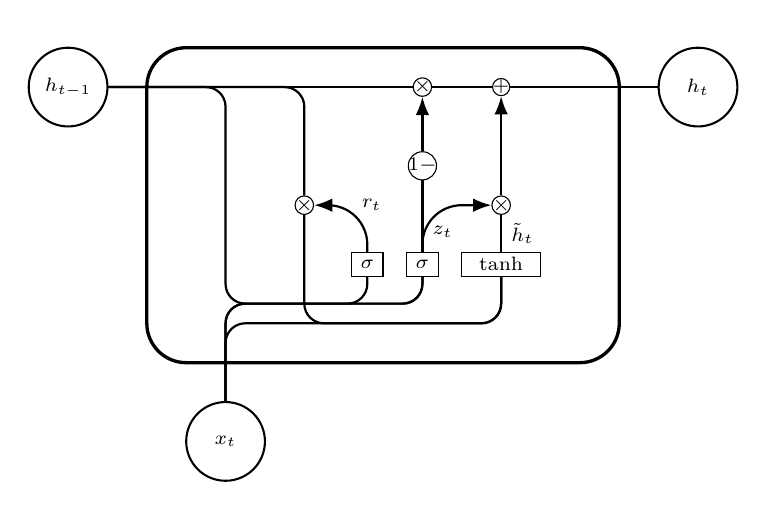
\begin{tikzpicture}[
    % GLOBAL CFG
    font=\sf \scriptsize,
    >=LaTeX,
    % Styles
    cell/.style={% For the main box
        rectangle, 
        rounded corners=5mm, 
        draw,
        very thick,
        },
    operator/.style={%For operators like +  and  x
        circle,
        draw,
        inner sep=-0.5pt,
        minimum height =.2cm,
        },
    function/.style={%For functions
        ellipse,
        draw,
        inner sep=1pt
        },
    ct/.style={% For external inputs and outputs
        circle,
        draw,
        line width = .75pt,
        minimum width=1cm,
        inner sep=1pt,
        },
    gt/.style={% For internal inputs
        rectangle,
        draw,
        minimum width=4mm,
        minimum height=3mm,
        inner sep=1pt
        },
    mylabel/.style={% something new that I have learned
        font=\scriptsize\sffamily
        },
    ArrowC1/.style={% Arrows with rounded corners
        rounded corners=.25cm,
        thick,
        },
    ArrowC2/.style={% Arrows with big rounded corners
        rounded corners=.5cm,
        thick,
        },
    ]

    % Draw the cell: 
    \node [cell, minimum height =4cm, minimum width=6cm] at (0,0){} ;

    % Draw inputs named ibox#
    \node [gt] (ibox1) at (-0.2,-0.75) {$\sigma$};
    \node [gt] (ibox2) at (0.5,-0.75) {$\sigma$};
    \node [gt, minimum width=1cm] (ibox3) at (1.5,-0.75) {$\tanh$};

   % Draw opérators   named mux# , add# and func#
    \node [operator] (mux1) at (-1,0) {$\times$};
    \node [operator] (mux2) at (0.5,1.5) {$\times$};
    \node [operator] (add1) at (1.5,1.5) {+};
    \node [operator] (-1) at (0.5,0.5) {$1-$};
    \node [operator] (mux3) at (1.5,0) {$\times$};

    \node[ct, label={[mylabel]}] (h0) at (-4,1.5) {$h_{t-1}$};
    \node[ct, label={[mylabel]}] (h1) at (4,1.5) {$h_{t}$};
    \node[ct, label={[mylabel]}] (x) at (-2,-3) {$x_t$};

    % Start connecting all.
    \draw [ArrowC1] (h0) -- (mux2) -- (add1) -- (h1);
    \draw [->, ArrowC1] (ibox2) -- (-1) -- (mux2);
    \draw [->, ArrowC1] (ibox3) -- (mux3) -- (add1);

    % Inputs
    \draw [ArrowC1] (h0) -| (mux1) -- (mux1 |- 0,-1.5)-| (ibox3);
    \draw [ArrowC1] (h0) -| (-2,-1.25) -- (mux1 |- 0,-1.25)-| (ibox2);
    \draw [ArrowC1] (x) -- (x |- 0,-1.25)-| (ibox1);
    \draw [ArrowC1] (x) -- (x |- 0,-1.25)-| (ibox2);
    \draw [ArrowC1] (x) -- (x |- 0,-1.5)-| (ibox3);
    \draw [ArrowC1] (ibox3) -- node[right] {$\tilde{h}_t$} (mux3);
    \draw [ArrowC1] (ibox2) -- node[right, yshift=-2mm] {${z}_t$} (-1);

    % Internal
    \draw [->, ArrowC2] (ibox1) |- node[right,xshift=-2mm] {$r_t$} (mux1);
    \draw [->, ArrowC2] (ibox2) |- (mux3);

  \end{tikzpicture}
  \caption{A GRU unit.}
  \label{grucell}
\end{figure}

 % corrected

\subsection{Production ($\pm$ 40\% of section's words)}
\textcolor{gray}{Provide descriptions of the deliverables concrete production.
It must present part of the deliverable (e.g. source code extracts, scientific
work extracts) to illustrate and explain its actual production.}

\subsubsection{Feature extraction with MFCC in Python}

% corrected LN 87

\subsection{Assessment}
\subsubsection{NFR01: Performance evaluation}~\label{assessment}~\\

In this section, the performance of the four ANNs investigated in
Section~\ref{ann} are evaluated. We use the English and Luxembourgish dataset
for the performance analysis.\\

The English and Luxembourgish dataset contains spoken words $w \in
\{'0',\dots,'9'\}$. The English dataset consists of 17749 data instances whereas
the Luxembourgish consists of 500 data instances.\\

The first step is to choose an optimal optimizer. The choice is between using
the stochastic gradient descent (SGD) or Adam optimizer. The latter is a
combination of two extensions of SGD, Adaptive Gradient Algorithm (AdaGrad) and
Root Mean Square Propagation (RMSProp)~\cite{Adam}. The four models will be
trained on the English dataset to designate the right optimizer and number of
epochs. Their training will be visualized with $60\ epochs$ each. The training
visualization is given in the appendix as follows:\\

\begin{enumerate}[label=\arabic*.]
  \item Feedforward Neural Network:
    \begin{itemize}
      \item Validation accuracy in Figure~\ref{ffa}.
      \item Validation loss in Figure~\ref{ffl}.
    \end{itemize}
  \item RNN:
    \begin{itemize}
      \item Validation accuracy in Figure~\ref{rnna}.
      \item Validation loss in Figure~\ref{rnnl}.
    \end{itemize}
  \item LSTM:
    \begin{itemize}
      \item Validation accuracy in Figure~\ref{lstma}.
      \item Validation loss in Figure~\ref{lstml}.
    \end{itemize}
  \item GRU:
    \begin{itemize}
      \item Validation accuracy in Figure~\ref{grua}.
      \item Validation loss in Figure~\ref{grul}.
    \end{itemize}
\end{enumerate}~\\

Let $n=60$ be the number of epochs. The two optimizers return the following
testing accuracies (acc) and losses:

\begin{table}[H]
    \centering
    \resizebox{\columnwidth}{!}{%
    \begin{tabular}{|c|c|c|c|c|c|c|c|c|}
        \hline
        \multirow{2}{*}{Optimizer} & \multicolumn{2}{c|}{FF} &
        \multicolumn{2}{c|}{RNN} & \multicolumn{2}{c|}{LSTM} &
        \multicolumn{2}{c|}{GRU} \\
        \cline{2-9}
        & {acc} & {loss} & {acc} & {loss} & {acc} & {loss} & {acc} & {loss}\\
        \hline
        SGD & 0.79 & 0.65 & 0.43 & 1.51 & 0.86 & 0.46 & 0.85 & 0.46 \\ \hline
        Adam & 0.87 & 0.47 & 0.72 & 0.97 & 0.94 & 0.24 & 0.94 & 0.24 \\ \hline
    \end{tabular}%
    \caption{Comparison of the four models' testing results using SGD and Adam.
    The models were trained on the English dataset.}
    \label{table:comparison}
    }
\end{table}

Table~\ref{table:comparison} shows that the validation accuracies using the Adam
optimizer yield better accuracies compared to SGD. Therefore, for the following
investigation, the Adam optimizer is considered.\\

The next step is to choose the number of epochs which will be used for the
performance analysis. The training visualizations show the loss converges around
$40$ epochs except for the RNN model. Figure \ref{300rnna} shows that the RNN
model converges around $220$ epochs with an accuracy of 0.88. The training
visualization of the RNN model with $300$ epochs is given in
Figures~\ref{300rnna} and~\ref{300rnnl} in the appendix.\\

Choosing $epochs = 40$ to evaluate each model's performance, we have:

\begin{table}[H]
    \centering
    \resizebox{\columnwidth}{!}{%
    \begin{tabular}{|c|c|c|c|c|c|c|c|c|}
        \hline
        \multirow{2}{*}{Optimizer} & \multicolumn{2}{c|}{FF} &
        \multicolumn{2}{c|}{RNN} & \multicolumn{2}{c|}{LSTM} &
        \multicolumn{2}{c|}{GRU} \\
        \cline{2-9}
                                 & {acc} & {loss} & {acc} & {loss} & {acc} &
        {loss} & {acc} & {loss}\\ \hline
        Adam & 0.83 & 0.54 & 0.63 & 1.10 & 0.937 & 0.23 & 0.94 &
        0.23 \\ \hline
    \end{tabular}%
    \caption{The testing results of the four models using Adam. The four models
    were trained on the English dataset. $FF$ is the abbreviation for feedforward
    and $acc$ stands for accuracy.}
    \label{table:40}
    }
\end{table}

Inspecting the results shows that LSTM and GRU perform better than feedforward
and RNN. The overall performance is slightly underneath the performance at 60
epochs. In this case, RNN has the lowest accuracy. This is expected, since
standard RNNs can't deal with learning long-term temporal dependencies, because
the gradient of the loss function decays exponentially with time (vanishing
gradient problem). LSTMs and GRUs use gated units to maintain the information in
memory for longer periods of time, and to control which information is kept, and
which is forgotten. This explains substantially better performance obtained
using LSTM and GRU. Compared to feedforward neural networks, LSTM and GRU have
better accuracy since they take advantage of their recurrent units to process
series data.\\

\textbf{Training on Luxembourgish dataset.} The same models used to train on the
English dataset were used to train on the Luxembourgish dataset. The following
testing accuracies and losses were obtained while training on the Luxembourgish
dataset:

\begin{table}[H]
    \centering
    \resizebox{\columnwidth}{!}{%
    \begin{tabular}{|c|c|c|c|c|c|c|c|c|}
        \hline
        \multirow{2}{*}{Optimizer} & \multicolumn{2}{c|}{FF} &
        \multicolumn{2}{c|}{RNN} & \multicolumn{2}{c|}{LSTM} &
        \multicolumn{2}{c|}{GRU} \\
        \cline{2-9}
        & {acc} & {loss} & {acc} & {loss} & {acc} & {loss} & {acc} & {loss}\\
        \hline
        Adam & 0.84 & 0.59 & 0.73 & 0.83 & 1.0 & 0.02 & 0.99 & 0.02 \\ \hline
    \end{tabular}%
    \caption{The testing results of the four models using Adam. The four models
    were trained on the Luxembourgish dataset. The dataset contains 50 instances
    of each spoken word. FF is the abbreviation for feedforward and $acc$ stands for
    accuracy.}
    \label{table:lux}
    }
\end{table}

The results show that LSTM and GRU generalize better than feedforward and RNN.
The validation accuracies of LSTM and GRU are both roughly 99\%. The high
accuracy of LSTM and GRU can be explained by the small dataset which is also
speaker-dependent.  The results of LSTM and GRU are expected to drop if the
dataset grows and contains a variety of speakers.\\

The training visualization on the Luxembourgish dataset is given in the appendix
as follows:\\

\begin{enumerate}[label=\arabic*.]
  \item Feedforward Neural Network:
    \begin{itemize}
      \item Validation accuracy in Figure~\ref{luxffa}.
      \item Validation loss in Figure~\ref{luxffl}.
    \end{itemize}
  \item RNN:
    \begin{itemize}
      \item Validation accuracy in Figure~\ref{luxrnna}.
      \item Validation loss in Figure~\ref{luxrnnl}.
    \end{itemize}
  \item LSTM:
    \begin{itemize}
      \item Validation accuracy in Figure~\ref{luxlstma}.
      \item Validation loss in Figure~\ref{luxlstml}.
    \end{itemize}
  \item GRU:
    \begin{itemize}
      \item Validation accuracy in Figure~\ref{luxgrua}.
      \item Validation loss in Figure~\ref{luxgrul}.
    \end{itemize}
\end{enumerate}

% corrected LN
\section{Technical Deliverables} 

As technical deliverables, the four ANN models are implemented in Python using
the Keras\cite{chollet2015keras} library and a small dataset containing
Luxembourgish spoken words is collected.

% corrected LN 100
\subsection{Requirements}

% -model implementation
% -luxembourgish data collection

\begin{itemize}
  \item \textbf{FR01} Implementation of the three classification models\\
    We use the Keras library to implement our models with three
    different Neural Network architecture
  \item \textbf{FR02} Collect a small dataset of Luxembourgish spoken words\\
    We collect a small dataset containing Luxembourgish audio samples containing
    the words $w \in \{'0',\dots,'9'\}$
\end{itemize}

% corrected LN 74

\subsection{Design}

% Keras api definition

\textit{Keras} is a high-level Neural Networks API written in Python. It is
designed for easy-to-use and efficient experimentation with Deep
Learning.~\cite{chollet2015keras}\\

% getting started

The main data structure in Keras is a model. The common model is the
\textit{Sequential} model which organizes layers in a linear stack. An example
of a \textit{Sequential} model in Python is given below:

\begin{lstlisting}
from keras.models import Sequential

model = Sequential()
\end{lstlisting}

\noindent To stack layers in the model, the \textit{.add()} function is used:

\begin{lstlisting}
from keras.layers import Dense

model.add(Dense(unit=64, activation='relu', 
                input_dim=100))
model.add(Dense(unit=10, activation='softmax'))
\end{lstlisting}

\noindent After stacking up the model, its learning process has to be configured
with \textit{.compile()} function:

\begin{lstlisting}
modl.compile(loss='categorical_crossentropy', 
             optimizer='sgd',
             metrics=['accuracy'])
\end{lstlisting}

\noindent Now the training data can be iterated in batches:

\begin{lstlisting}
model.fit(x_train, y_train, epochs=5, batch_size=32)
\end{lstlisting}

\noindent To evaluate the performance of the model, the \textit{.evaluate()}
function is called:

\begin{lstlisting}
loss_and_metrics = model.evaluate(x_test, y_test, batch_size=128)
\end{lstlisting}

\subsection{Production}

% corrected LN 86
\subsubsection{Implementation of classification models}\label{implementation}~\\

In this section, the implementation of the four ANN models are presented.\\

First of all, we initialize the training and testing sets:
\lstinputlisting{sections/technical/fr1/input.py}

\begin{enumerate}[label=\arabic*.]
  \item Feedforward:
    \lstinputlisting{sections/technical/fr1/feedforward.py}
    The sequential model is used to stack four \textit{Dense} layers. The first
    dense layer takes as input a vector with the same dimensions as a row in the
    dataset. The first three layers are using \textit{ReLU} as activation
    function whereas the output layer is using \textit{softmax}. In between the
    dense layers, dropout layers are stacked. Theses dropout layers are dropping
    units from the model to prevent overfitting. The parameter \textit{loss} of
    the \textit{.compile()} function is set to
    \textit{'sparse\_categorical\_crossentropy'} which sets the model to take in
    1D vectors instead of a matrix.\\

  \begin{normalize}
    Before continuing with the recurrent models, the input data has to be
    reshaped since RNN, LSTM and GRU are taking in 3D shaped input data:
    \lstinputlisting{sections/technical/fr1/inputchange.py}~\\
  \end{normalize}
  \item RNN:
    \lstinputlisting{sections/technical/fr1/rnn.py}
    The RNN model is implemented in the same manner as the feedforward model.
    Instead of using dense layers, this model uses \textit{SimpleRnn} layers.
    The parameter \textit{return\_sequences} is set to \textit{True} so that the
    next simpleRNN layer has access to all the hidden states from the previous
    layer.  The output layer is again a dense layer with \textit{softmax} as the
    activation function. As input, it takes in a matrix, which is an instance of
    the 3D dataset.~\\

  \item LSTM:
    \lstinputlisting{sections/technical/fr1/lstm.py}
    The LSTM model uses \textit{LSTM} layers. Its parameter
    \textit{return\_sequences} is set to \textit{True} with the same reason as
    for the RNN model. The LSTM model has the same output layer as the two
    previous ones.\\
  \item GRU:
    \lstinputlisting{sections/technical/fr1/gru.py}
    The GRU model uses \textit{GRU} layers. Its parameters are set to the same
    values as the RNN and LSTM model. It uses the same dense layer activated by
    the \textit{softmax} function as output layer.
\end{enumerate}

% corrected LN 83

\subsubsection{FR02: Luxembourgish dataset collection}~\\

To collect the Luxembourgish dataset, the \textit{Teachable
Machine}\cite{teachablemachine} was used. It contains a recorder to create a
dataset consisting of audio files. The recording of the audio files can be set
to $1s$. However, the recorder saves the files in the \textit{.webm} file type.
Therefore, the audio files have to be converted to \textit{.wav} files before
the features can be extracted. The following bash script using the
\textit{ffmpeg} command converts the audio files in a file directory to the
desired file format:

\lstset{
  language = Bash,
  literate = {\#\#}{{{\#\#}}}2,
  columns  = fullflexible,
  keepspaces,
}

\newpage

\lstinputlisting[language=Bash]{sections/technical/fr2/ffmpeg.sh}


\subsection{Assessment ($\pm$ 15\% of section's words)}

% corrected LN 96
\section*{Acknowledgment}
I would like to thank my tutor Vladimir Despotovic for his constructive feedback and
mentorship. His introduction and explanation of neural networks were outstanding. I
would recommend fellow BiCS Students interested in this field to work with
Vladimir Despotovic. Additionally, I thank him for supervising my paper.


% corrected LN 74

\section{Conclusion}

In this paper, end-to-end isolated word recognition using deep neural networks
is presented. Four different ANN models were investigated. The focus of this
paper is using RNN architectures for end-to-end speech recognition and
investigating whether gated RNNs outperform vanilla RNN units and how they deal
with long-term dependencies. The results showed, that gated RNNs substantially
outperform basic feedforward and recurrent neural networks. The performance
analysis can be consulted in Section~\ref{assessment}\\

A further objective of this paper is to recognize Luxembourgish words. To the
best of our knowledge, there is a lack of continuous speech dataset in
Luxembourgish. Thus efforts were put to collect a small dataset containing
Luxembourgish spoken words $w \in \{'Null',\dots,'Neng'\}$. This dataset was
recorded by one person which makes it speaker-dependent speech recognition. In
Section~\ref{datasetlux} the methods used to collect the dataset were
elaborated. Four previously discussed ANN architectures were applied to our
collected Luxembourgish dataset and yielded excellent performance with accuracy
close to 1.\\

Continuation of this project would be to extend the Luxembourgish dataset with
continuous speech or to add instances spoken by multiple speakers.\\

In my opinion, I find it interesting to work with deep neural networks and their
practical use. This project will give me the required background to start on my
next BSP which deals with attention-based models for speech recognition.

\bibliography{BSPS3}
\bibliographystyle{IEEEtran}

\onecolumn
\newpage
\clearpage
\section{Appendix}

% \begin{enumerate}[label=\arabic*.]
%   \item Feedforward:
    \begin{figure}[h]
      \centering
      \subfloat[Feedforward'accuracy using SGD, although SGD didn't work well.]{{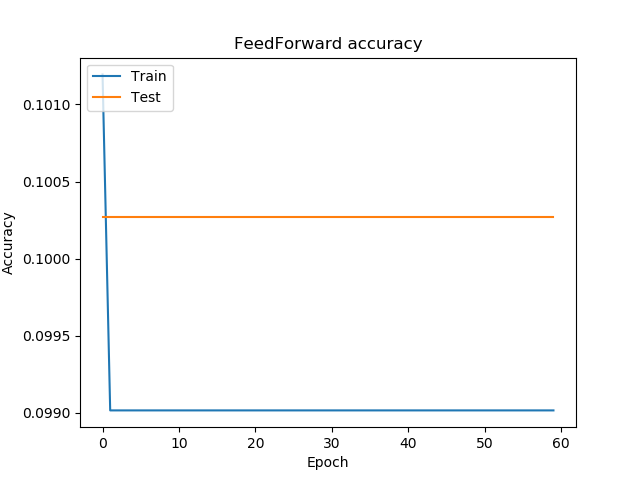
\includegraphics[scale=0.5]{sgdffa.png} }}%
      \qquad
      \subfloat[Feedforward'accuracy using Adam.]{{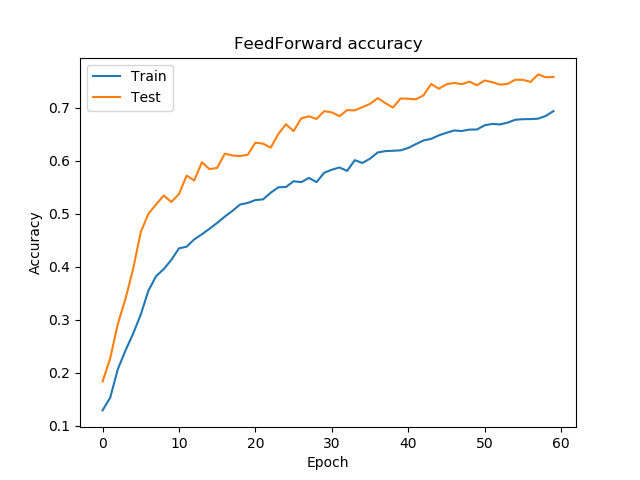
\includegraphics[scale=0.5]{adamffa.png} }}%
      \caption{Accuracy comparison between feedforward using SGD and Adam.}%
      \label{ffa}
    \end{figure}
    \begin{figure}[h]
      \centering
      \subfloat[Feeforward'loss using SGD, loss returns NaN.]{{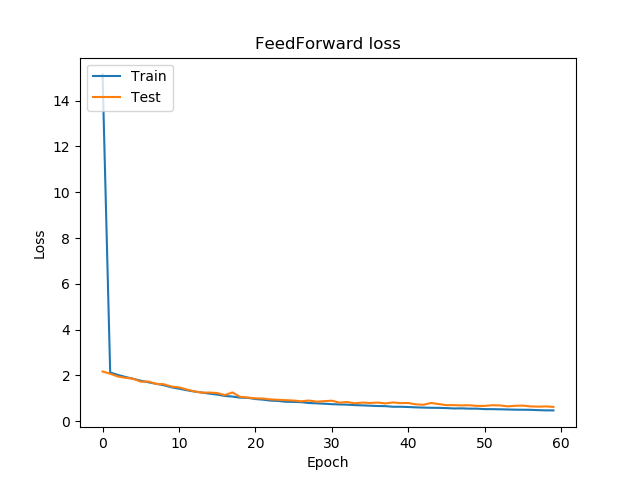
\includegraphics[scale=0.5]{sgdffl.png} }}%
      \qquad
      \subfloat[Feeforward'loss using Adam.]{{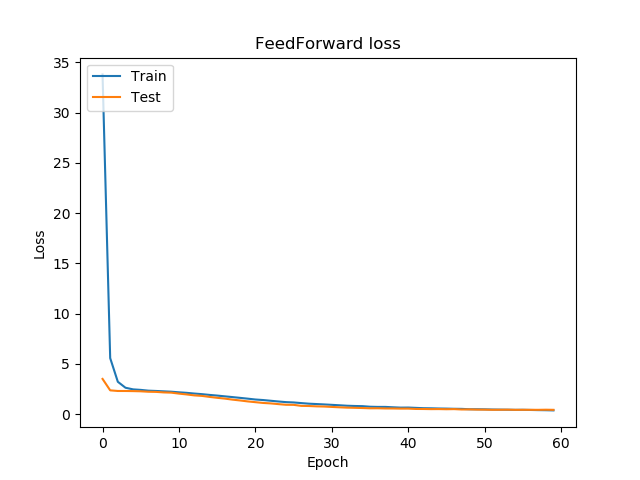
\includegraphics[scale=0.5]{adamffl.png} }}%
      \caption{Loss comparison between feedforward using SGD and Adam.}%
      \label{ffl}
    \end{figure}
  % \item RNN:
    \begin{figure}[h]
      \centering
      \subfloat[RNN's accuracy using SGD.]{{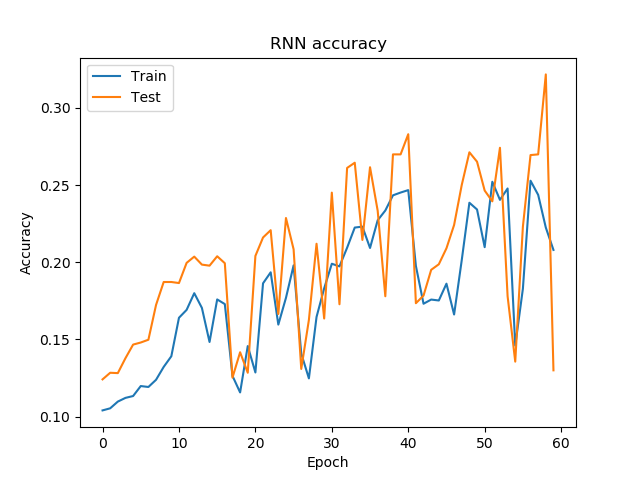
\includegraphics[scale=0.5]{sgdrnna.png} }}%
      \qquad
      \subfloat[RNN's accuracy using Adam.]{{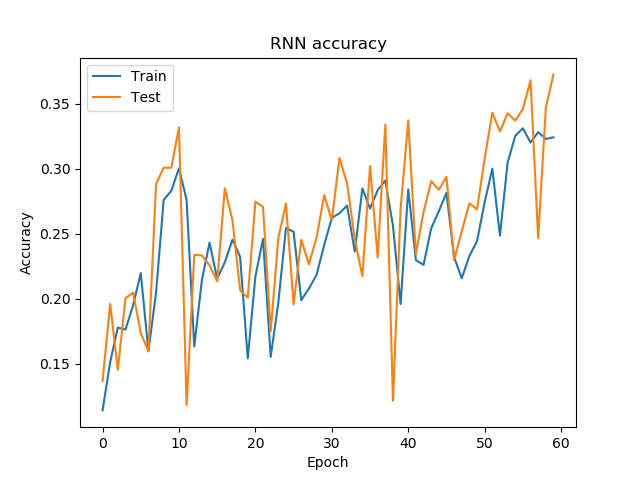
\includegraphics[scale=0.5]{adamrnna.png} }}%
      \caption{Accuracy comparison between RNN using SGD and Adam.}%
      \label{rnna}
    \end{figure}
    \begin{figure}[h]
      \centering
      \subfloat[RNN's loss using SGD.]{{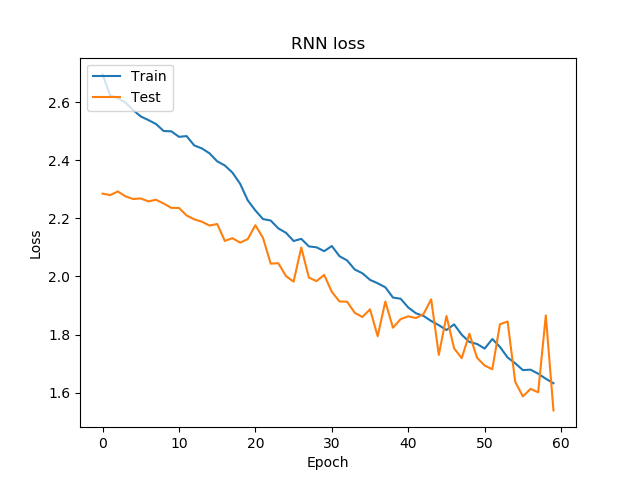
\includegraphics[scale=0.5]{sgdrnnl.png} }}%
      \qquad
      \subfloat[RNN's loss using Adam.]{{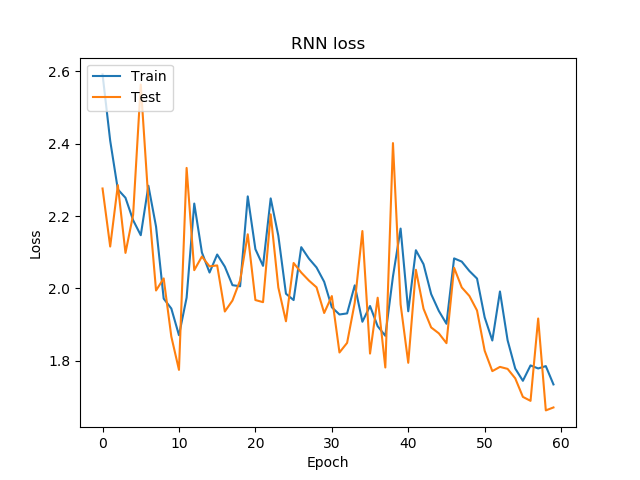
\includegraphics[scale=0.5]{adamrnnl.png} }}%
      \caption{Loss comparison between RNN using SGD and Adam.}%
      \label{rnnl}
    \end{figure}
  % \item LSTM:
    \begin{figure}[h]
      \centering
      \subfloat[LSTM's accuracy using SGD.]{{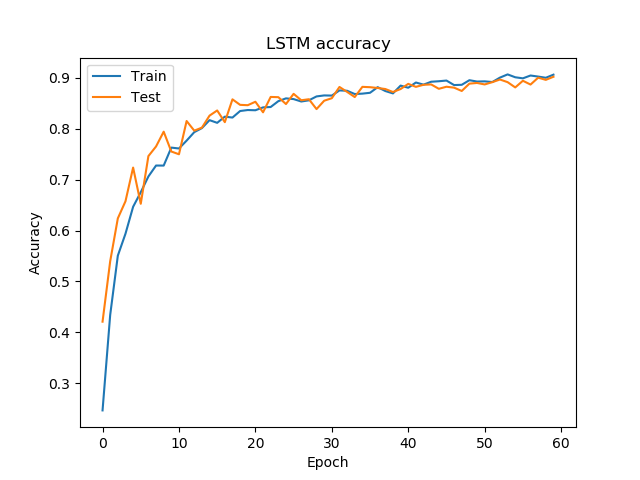
\includegraphics[scale=0.5]{sgdlstma.png} }}%
      \qquad
      \subfloat[LSTM's accuracy using Adam.]{{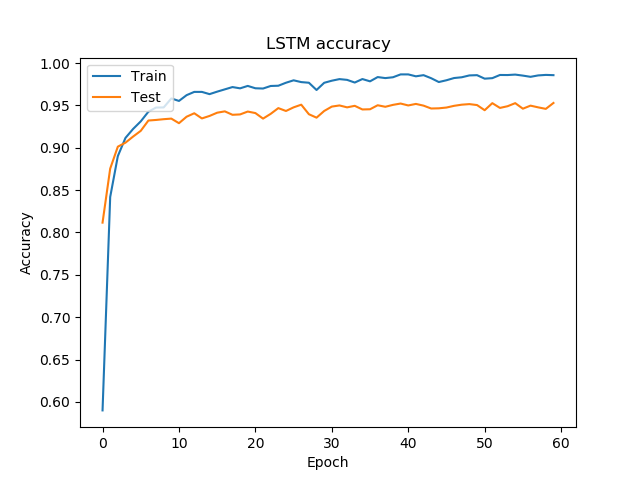
\includegraphics[scale=0.5]{adamlstma.png} }}%
      \caption{Accuracy comparison between RNN using SGD and Adam.}%
      \label{lstma}
    \end{figure}
    \begin{figure}[h]
      \centering
      \subfloat[LSTM's loss using SGD.]{{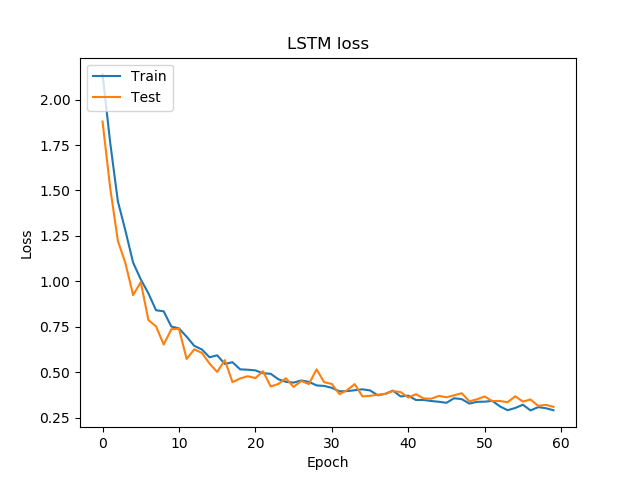
\includegraphics[scale=0.5]{sgdlstml.png} }}%
      \qquad
      \subfloat[LSTM's loss using Adam.]{{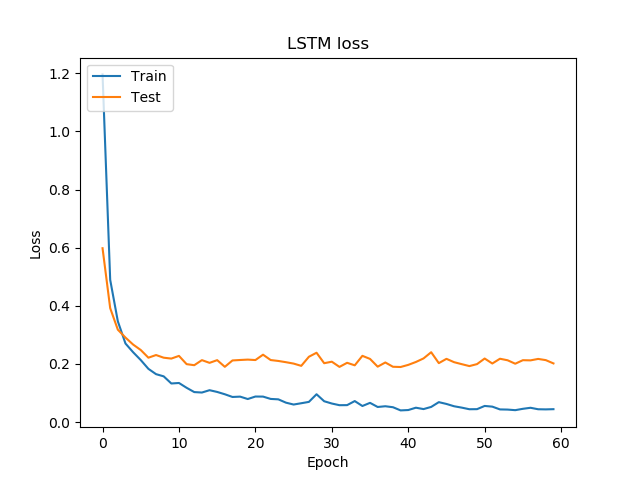
\includegraphics[scale=0.5]{adamlstml.png} }}%
      \caption{Loss comparison between LSTM using SGD and Adam.}%
      \label{lstml}
    \end{figure}
  % \item GRU:
    \begin{figure}[h]
      \centering
      \subfloat[GRU's accuracy using SGD.]{{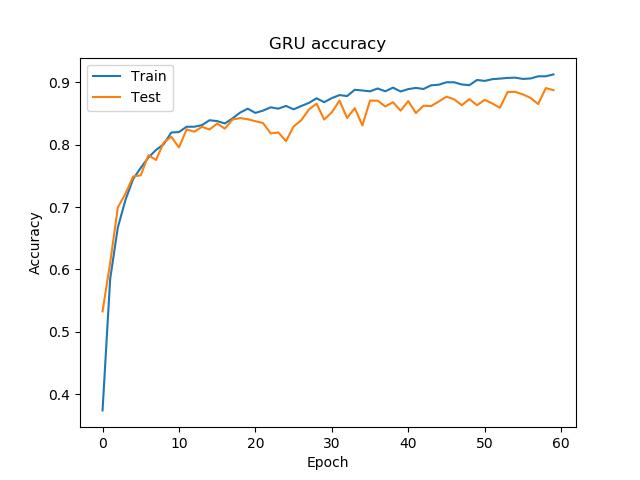
\includegraphics[scale=0.5]{sgdgrua.png} }}%
      \qquad
      \subfloat[GRU's accuracy using Adam.]{{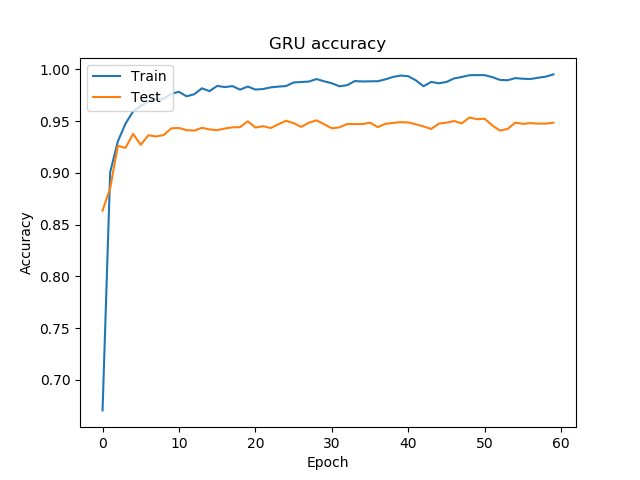
\includegraphics[scale=0.5]{adamgrua.png} }}%
      \caption{Accuracy comparison between RNN using SGD and Adam.}%
      \label{grua}
    \end{figure}
    \begin{figure}[h]
      \centering
      \subfloat[GRU's loss using SGD.]{{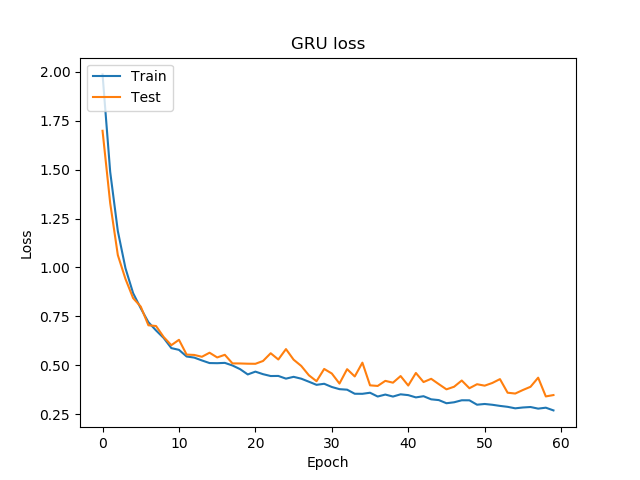
\includegraphics[scale=0.5]{sgdgrul.png} }}%
      \qquad
      \subfloat[GRU's loss using Adam.]{{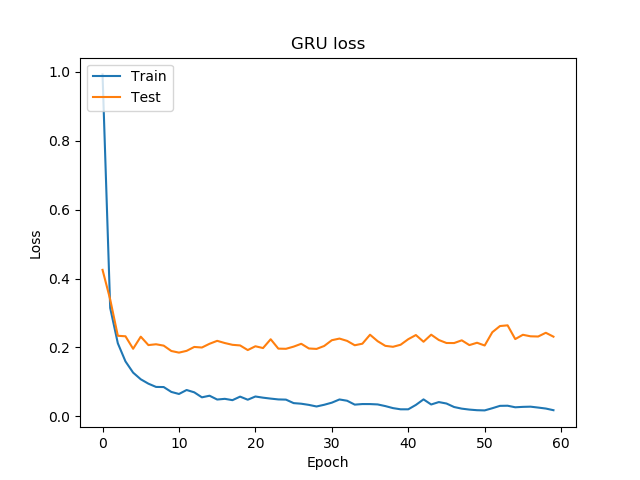
\includegraphics[scale=0.5]{adamgrul.png} }}%
      \caption{Loss comparison between GRU using SGD and Adam.}%
      \label{grul}
    \end{figure}
% \end{enumerate}

\begin{figure}[h]
  \centering
  \lstinputlisting{sections/scientific/fr1/mfccsnippet.py}
  \caption{Code snippet to extract MFCCs from the dataset.}
  \label{mfccsnip}
\end{figure}


\end{document}
